\chapter{Zanarkand}
\begin{enumerate}
  \item \sd, \cs[0:50], walk left. \fmv+\cs[2:20]
  \item Move left to the sphere, \sd, \cs[1:40]. Walk further left and follow the path down, \pickup{Fortune Sphere} on the left of the road. \cs[3:20], walk left onto the next screen.
  \item Make sure that you build up \rikku\ \od\ for the final boss
  \item If you missed the Overkill on \textbf{Seymour Flux}, then kill two \textbf{YKT-11} with \yuna\ and \tidus.
  \item Continue on the path. Seymour's Mom \cs, \pickup{Friend Sphere} on the right. When you leave the last encounter zone, \pickup{Luck Sphere}
\end{enumerate}
\end{multicols}
\begin{spheregrid}
  \begin{multicols}{2}
    \begin{itemize}
      \item Activate a Luck Sphere and a Fortune Sphere at some point during this Sphere Grid
            \yunaf
            \begin{itemize}
              \item \textit{If you got \textbf{4 Return Spheres}:}
                    \begin{itemize}
                      \item Friend Sphere to \lulu
                      \item Luck Sphere, Fortune Sphere
                      \item Str+4, Str+4
                      \item Move to Str+3
                      \item Agi+4, Agi+4, Str+3
                      \item Return to Mag+3 in \wakka's grid ($\uparrow, \rightarrow, \downarrow$)
                      \item Move down one node
                      \item Str+2
                    \end{itemize}
                    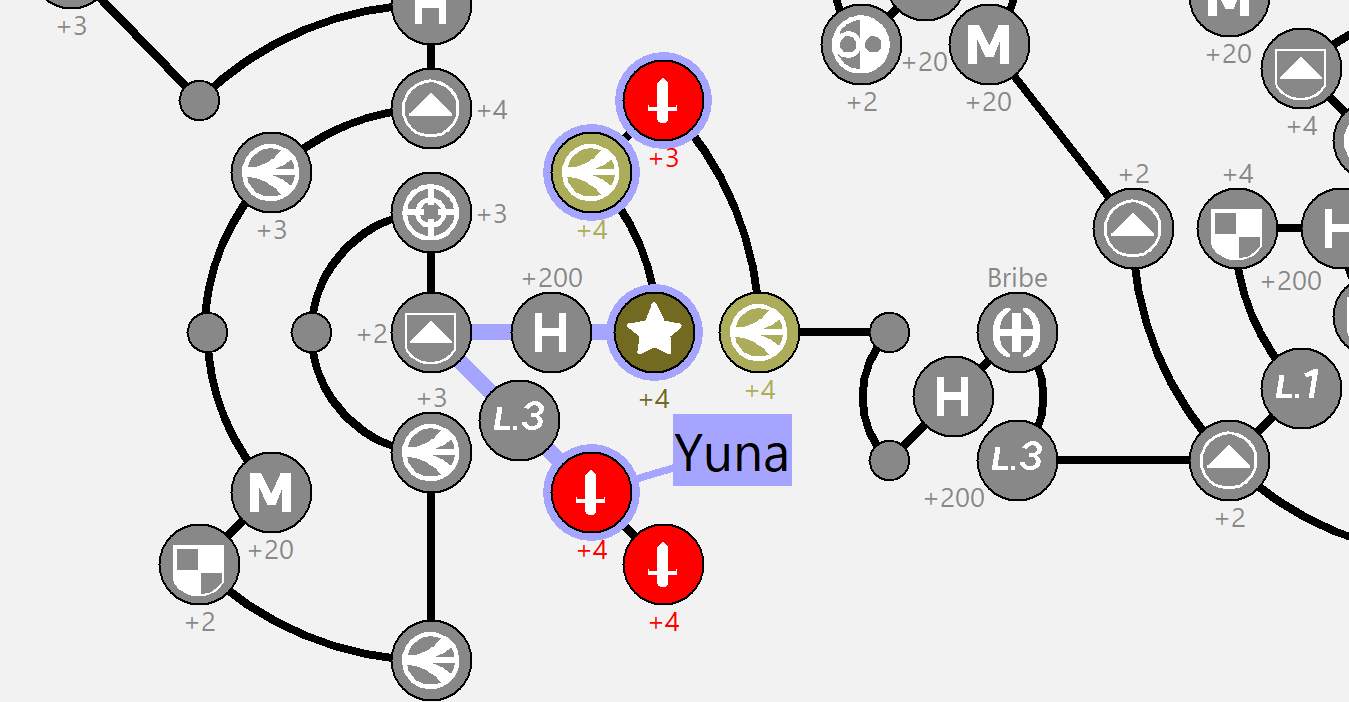
\includegraphics[width=.5\columnwidth]{graphics/4_returns_w_luck_pt1}
                    \newline
                    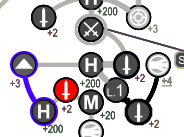
\includegraphics[width=.5\columnwidth]{graphics/4_returns_w_luck_pt2}
                    \columnbreak
              \item \textit{If you got \textbf{2 Return Spheres}:}
                    \begin{itemize}
                      \item Return to Str+2 in \wakka's grid
                      \item Move to HP node
                      \item Mag+3, Level 1 Key Sphere, STr+2, Agi+4
                      \item Luck Sphere, Fortune Sphere
                      \item Move back down
                      \item Str+2, Str+2, Agi+3
                    \end{itemize}
                    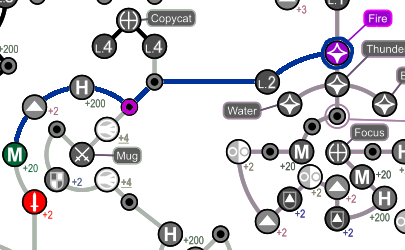
\includegraphics[width=.5\columnwidth]{graphics/2_and_2_with_luck}
              \item \textit{If you got \textbf{0 Return Spheres}:}
                    \begin{itemize}
                      \rikkuf Move to the MDef Node below Agi+4 below you
                      \yunaf Friend Sphere to \rikku
                      \item Agi+4, Spare Change, Agi+4
                    \end{itemize}
                    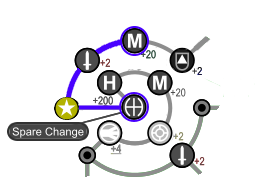
\includegraphics[width=.7\columnwidth]{graphics/0_return_w_luck}
            \end{itemize}
    \end{itemize}
  \end{multicols}
\end{spheregrid}
\begin{multicols}{2}
\begin{enumerate}[resume]
  \item \textit{If you're doing Quick Hit endgame:} If \rikku\ doesn't have 30 levels, give her a turn in the next fight
  \item \formation{\tidus}{\yuna}{\auron}
  \item \save
\end{enumerate}
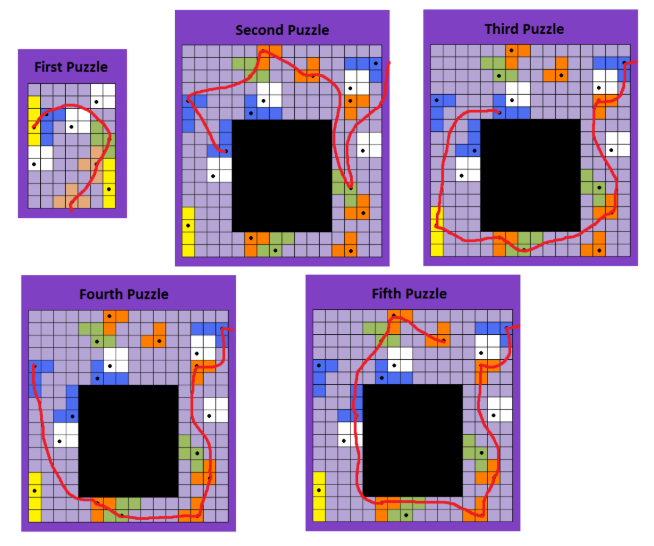
\includegraphics[scale=.8]{graphics/zanarkandpuzzles}
\begin{enumerate}[resume]
  \item After the fifth puzzle, take the Besaid Sphere and place it into the fifth pedestal and push it in
  \item \cs, run into the large room
\end{enumerate}
\begin{battle}[52000]{Spectral Keeper}
  \begin{itemize}
    \summon{\bahamut}
    \bahamutf Attack
  \end{itemize}
\end{battle}
\begin{spheregrid}
  \begin{itemize}
    \item \textit{If you had 4 \textbf{Return Spheres}}: Agi+3, Str+2
    \item \yuna\ should have 70 Str and 35 Agi. If short, then the key Str Nodes are near \tidus's Armor Break and the end of \wakka's grid, and Agi is near \lulu\ (+8), \rikku\ (+3) and \wakka (+3 near Mag+3). If you need more Return Spheres to do these, then you can attack Sinspawn Genesis for an extra one, though it costs 26 seconds
  \end{itemize}
  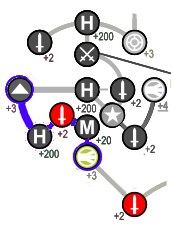
\includegraphics[width=.5\columnwidth]{graphics/4_return_before_yunalesca}
\end{spheregrid}
\begin{enumerate}[resume]
  \item \save, Run up, \sd, walk up to Yunalesca's room, \sd
\end{enumerate}
\begin{battle}[132000]{Yunalesca}
  \begin{itemize}
    \summon{\bahamut}
    \bahamutf Attack
  \end{itemize}
  Check for any weapon drops with \textbf{Zombie Strike}
\end{battle}
\begin{enumerate}[resume]
  \item \sd, leave room, walk down steps, \sd, go down on the next screens, \save, go up the lift, walk out of the cloister of trials, walk down the steps, walk down, \sd during \cs+\skippablefmv
\end{enumerate}